\documentclass{article}
\usepackage{graphicx}
\usepackage{mathtools}
\usepackage{xfrac}
\usepackage{amsmath, amssymb}
\usepackage{listings}
\usepackage{float}
\usepackage{wrapfig}
\usepackage{tikz}
\usepackage{fullpage}
\usepackage{hyperref}
\usepackage{mathalpha}
\usepackage{tikz}
\usepackage{cite}
\usepackage{amsthm}
\usepackage{braket}
\usepackage[utf8]{inputenc}
\usepackage[T1]{fontenc}


\newtheorem{theorem}{Proposition}[section]
\newtheorem{corollary}{Corollary}[theorem]
\newtheorem{lemma}[theorem]{Lemma}

\theoremstyle{definition}
\newtheorem{definition}{Definition}[section]

\theoremstyle{remark}
\newtheorem*{remark}{Remark}
\newtheorem*{example}{Example}
\newtheorem*{notation}{Notation}

\title{Computational Simulation I: Python\\Assignment 3\\Exploring the 2D Ising Model, and the Use of Artificial Intelligence in Computational Physics}
\author{David Lawton\\22337087}
\date{16. Dec 2024.}

\begin{document}

\maketitle

\tableofcontents
\section{Introduction \& Theory}
This experiment studied several physical properties of the 2D Ising model, using Python, as well as assessing the use of generative AI in computational physics.
\subsection{The 2D Ising Model}
The Ising Model is a model of a ferromagnetic material, consisting of a lattice of spin-$\sfrac{1}{2}$ particles, which can be in one of two states, s=$\pm 1$. This system is one with constant temperature, volume and number of particles, and is in thermal equilibrium. We thus use the canonical ensemble, and partition function to describe the system. The energy of the system in some state $\alpha_j$ is distributed according to the Boltzmann distribution
\begin{equation}
    \label{eq: boltzmann}
    P(\alpha_j) = \frac{e^{-\beta E_j}}{Z}, \quad Z = \sum_{\alpha_j} e^{-\beta E_j}
\end{equation}
where $\beta = \frac{1}{kT}$, is the thermodynamic beta, $Z$ is the partition function, and $E_j$ is the energy of the system in state $\alpha_j$, which is defined by
\begin{equation}
    \label{eq: isingenergy}
    E_j = -J\sum_{i,j=1}^{N-1} s_{ij}S_{ij} - B\mu_b\sum_{i,j=1}^{N}s_{ij}, \quad S_{ij} = s_{i+1,j} + s_{i-1,j} + s_{i,j+1} + s_{i,j-1}
\end{equation}
for a 2D Ising Model with $N^2$ spins, $J$ is the coupling constant, $B$ is the magnetic field, and $\mu_b$ is the Bohr magneton. We use units here such that $J = 1$, and write $B\mu_b = h$ for an external magnetic field. This also means that thermal temperature $kT$ and energy $E$ are in units of $J$.\\
We can then define the magnetization $M$, heat capacity $C_v$, and magnetic susceptibility $\chi$ as
\begin{equation}
    \label{eq: mag,magsus,haetcap}
    M = \sum_{i,j=1}^{N}s_{ij}, \quad C_v \approx\frac{(\Delta E)^2}{\beta^2}, \quad \chi\approx\frac{(\Delta M)^2}{\beta}
\end{equation}
where $\Delta E$ and $\Delta M$ are the variance of energy and magnetization of the system over many iterations. We can then use the Metropolis algorithm to sample the Boltzmann distribution and calculate $\braket{E},\braket{M},\chi,C_v$ for given $h, kT$ values.\\
\indent The reason for studying the 2D Ising model is that given some ferromagnetic material, with a given structure, we can an Ising model with the same structure to predict the behaviour of the material in varying conditions. By using periodic or finite boundary conditions, we can also study the bulk or surface properties of the material, respectively.\\
\subsection{Metropolis Algorithm}
The Metropolis algorithm is a MCMC method for sampling a probability distribution. The algorithm is used in this experiment by flipping the spin of some particle, meausuring the change in energy of the system, and then either accepting or rejecting the flip based on the Boltzmann distribution.
\begin{equation}
    \label{eq: metropolis}
    \delta E = 2s_{ij}S_{ij} + 2h, \quad P(\delta E) = \mathrm{min}(1, e^{-\beta\delta E})
\end{equation}
where $\delta E$ is the change in energy of the system sue to the flip, and $P(\delta E)$ is the probability of accepting the spin flip. $N^2$ flips are performed, either at random or sequentially, across the grid, in what we call a sweep. We then measure the energy and magnetization of the system, as well as these quantities squared. After performing many sweeps, the expectation values of $M$, $E$ and their squares converge to the true values, and we can calculate $C_v$, $\chi$ from these. In this experiment we started off using a square grid of side $N=10$, with periodic boundary conditions.\\
\subsection{Generative AI}
Generative AI refers to computational techniques which, from training data, can generate `seemingly new,
meaningful content such as text, images, or audio'. Generative AI aims to fit data to a probability distribution, and then sample from this distribution to generate new.
\section{Methodology}
The procedure for this experiment began with prompting the generative AI with the following:\\
\begin{center}
\textit{`Generate a Python class to simulate the 2D Ising model on a square lattice using the Metropolis Monte Carlo algorithm'}\\
\end{center}

The AI then generated a class modelling a 2D Ising model using Metropolis Algorithm, with methods for calculating the energy and magnetization of the lattice with periodic boundary conditions. The AI used an algorithm which randomly selects $N^2$ lattice points to flip the spins of using the following method.
\begin{lstlisting}[language=Python]
    def step(self):
        """Perform a single Metropolis step."""
        for _ in range(self.size ** 2):
            i = random.randint(0, self.size - 1)
            j = random.randint(0, self.size - 1)
            delta_E = self._delta_energy(i, j)
            if delta_E < 0 or random.random() < np.exp(-delta_E * self.beta):
                self.lattice[i, j] *= -1
\end{lstlisting}
The AI also did not consider the addition of an external field $h$ to the model, and so this was added afterward as an attribute of the class, and also the external field factor was added into the energy calculation . The AI also did not include methods for calculating the heat capacity and magnetic susceptibility, so these were also added as described in Eq.\ref{eq: mag,magsus,haetcap}.\\
\indent To improve the execution following tasks, we add a procedure to help us find the number of sweeps needed to reach an acceptable level of convergence to true values. This was done by running the simulation for varying numbers of sweeps, and plotting values of $\braket{E}$, $\braket{M}$, for each number of sweeps. The number of sweeps used for the remainder of the experiment was then chosen at a point such that a reasonable level of convergence had been reached, and the number of sweeps required does not itself require an overly large computation time.\\ 
\indent The next task was to, at constant temperatures, monitor the change of our system's observables ($\braket{E},\braket{M},\chi,C_v$) as a function of the external field $h$. This was done as described in the introduction.\\
\indent The system was then simulated at varying temperatures, for $h=0$, and the same variables were observed. The critical temperature can be observed as the temperature at which the heat capacity peaks ($E$ inflection point), and the magnetic susceptibility diverges.\\
\indent The final task was to use the AI to plot the magnetic susceptibilty $\chi$ and heat capacity $C_v$ as a function of system size for temperature near the critical temperature and 
\section{Results}
The first result is the convergence of the system to the true values of the means of energy and magnetization. As in Fig.\ref{fig: convergence}, the system reaches a realistic level of convergence to the thermodynamic limit after approximately 8000 sweeps. While the results would be more accurate for more sweeps, the significant increase in computation time which is required makes this extremely inefficient.\\
\begin{figure}
    \centering
    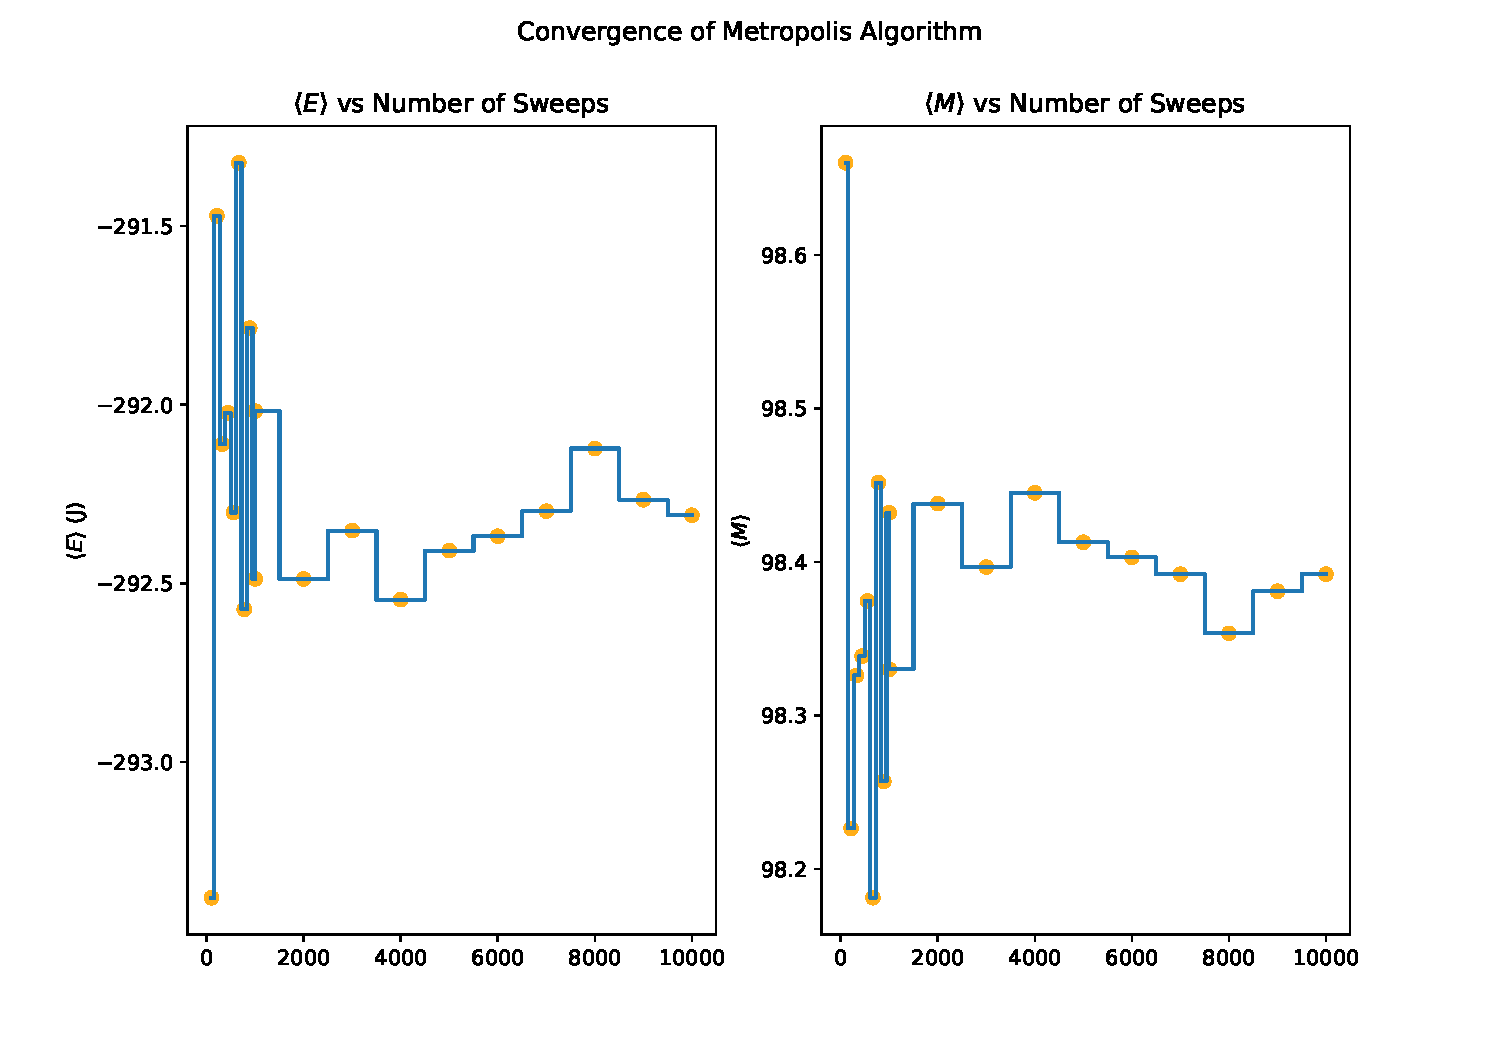
\includegraphics[width=0.6\textwidth]{convergence.pdf}
    \caption{\label{fig: convergence}Convergence of $\braket{E},\braket{M}$ as a function of number of sweeps for constant $kT$, $h$, $L=10$}
\end{figure}
The next result corresponds to variables as functions of $h$, at constant temperatures, as in Fig.\ref{fig: h_graph_T=1.0,4.0}. The magnetization clearly increases toward total polarisation ($\braket{M}=N$) as $h$ increases, and the minimum energy decreases linearly with $h$. The heat capacity and magnetic susceptibility both peak near $h=0$, and decrease as $h$ increases. The clear difference between the different temperature lies in the speed with which the lattcie reaches total polarisation, and the magnitude of the magnetic susceptibility. As well as this the heat capacity at $kT=4.0$ goes toward zero for small $h$, whereas at $kT=1.0$ it diverges for small $h$.\\
\begin{figure}
    \begin{flushleft}
    \begin{tabular}{cc}
    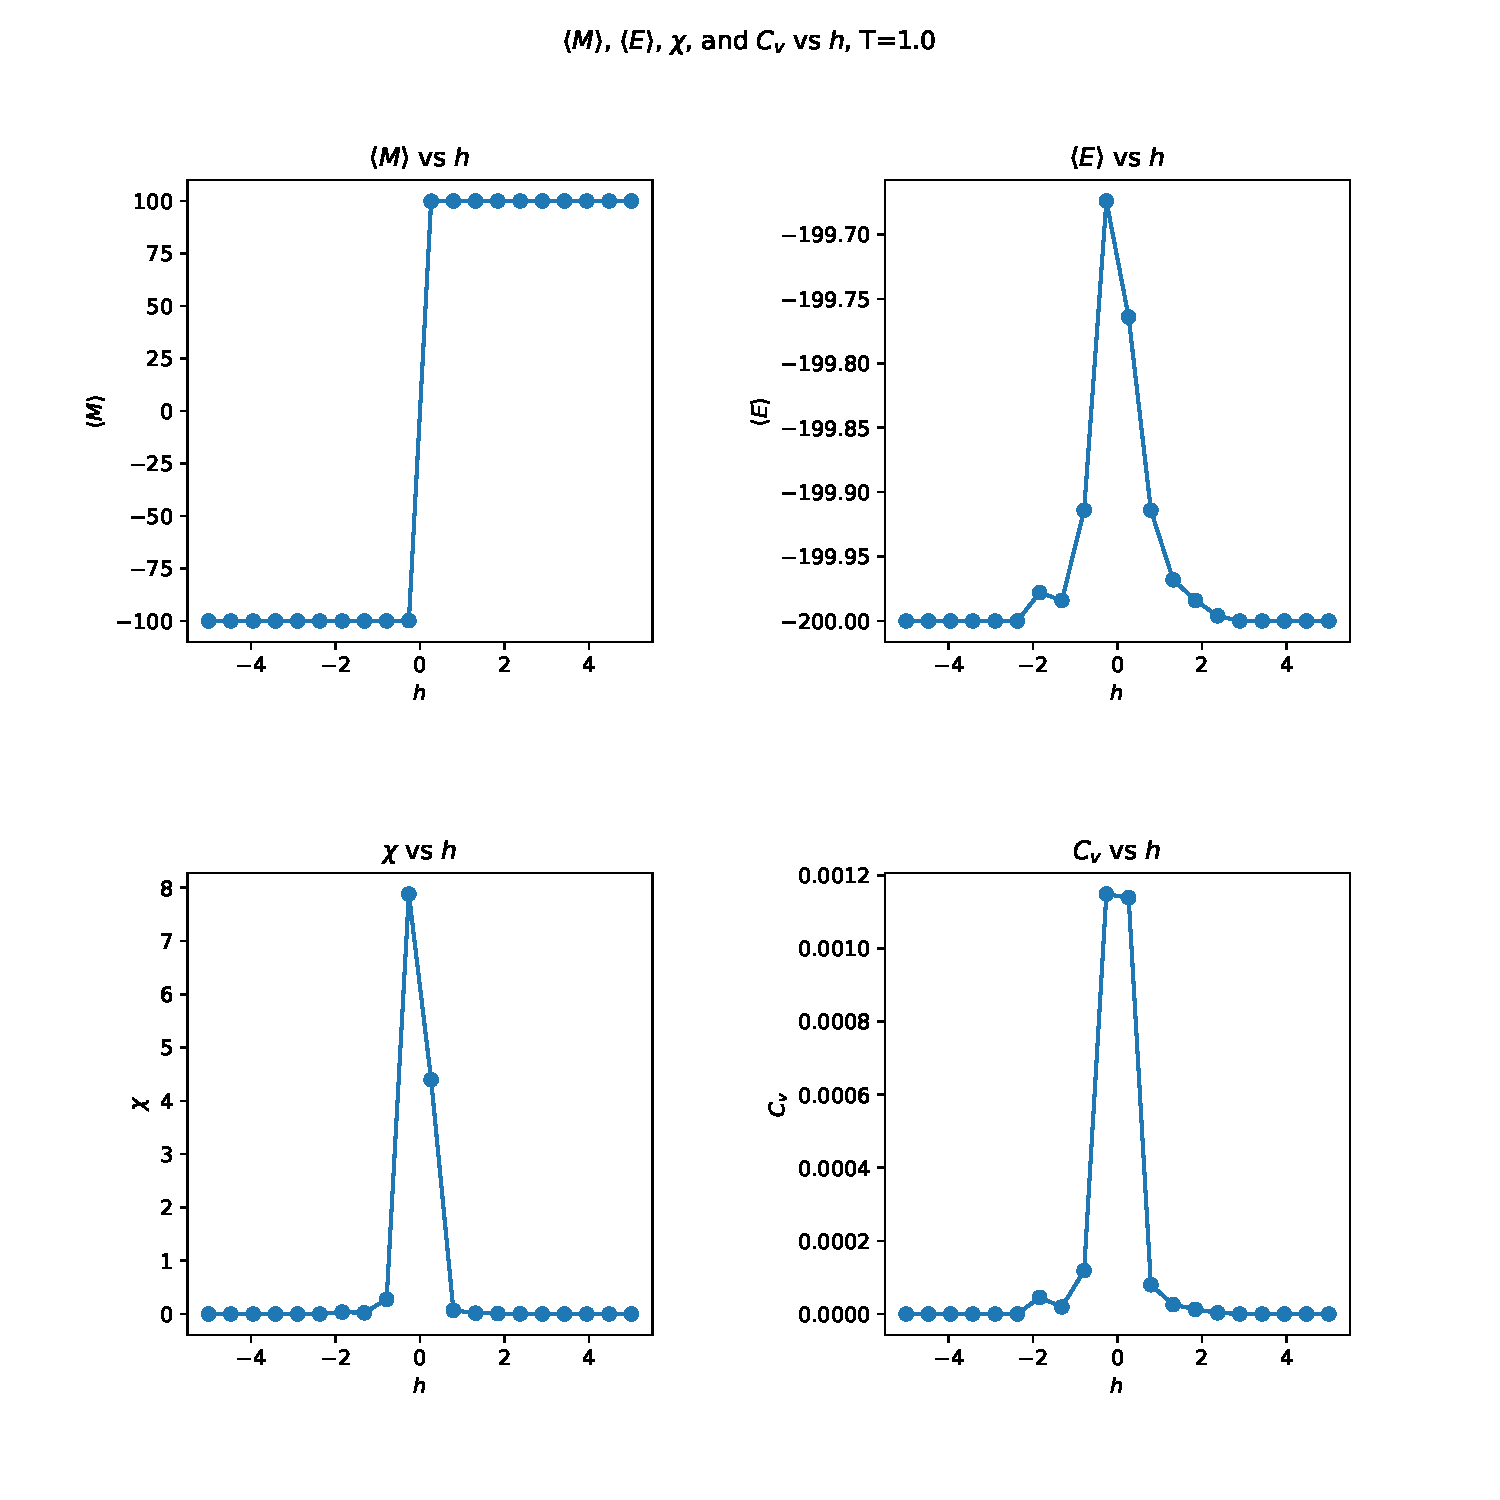
\includegraphics[width=0.5\textwidth]{h_graph_T=1.0.pdf} & 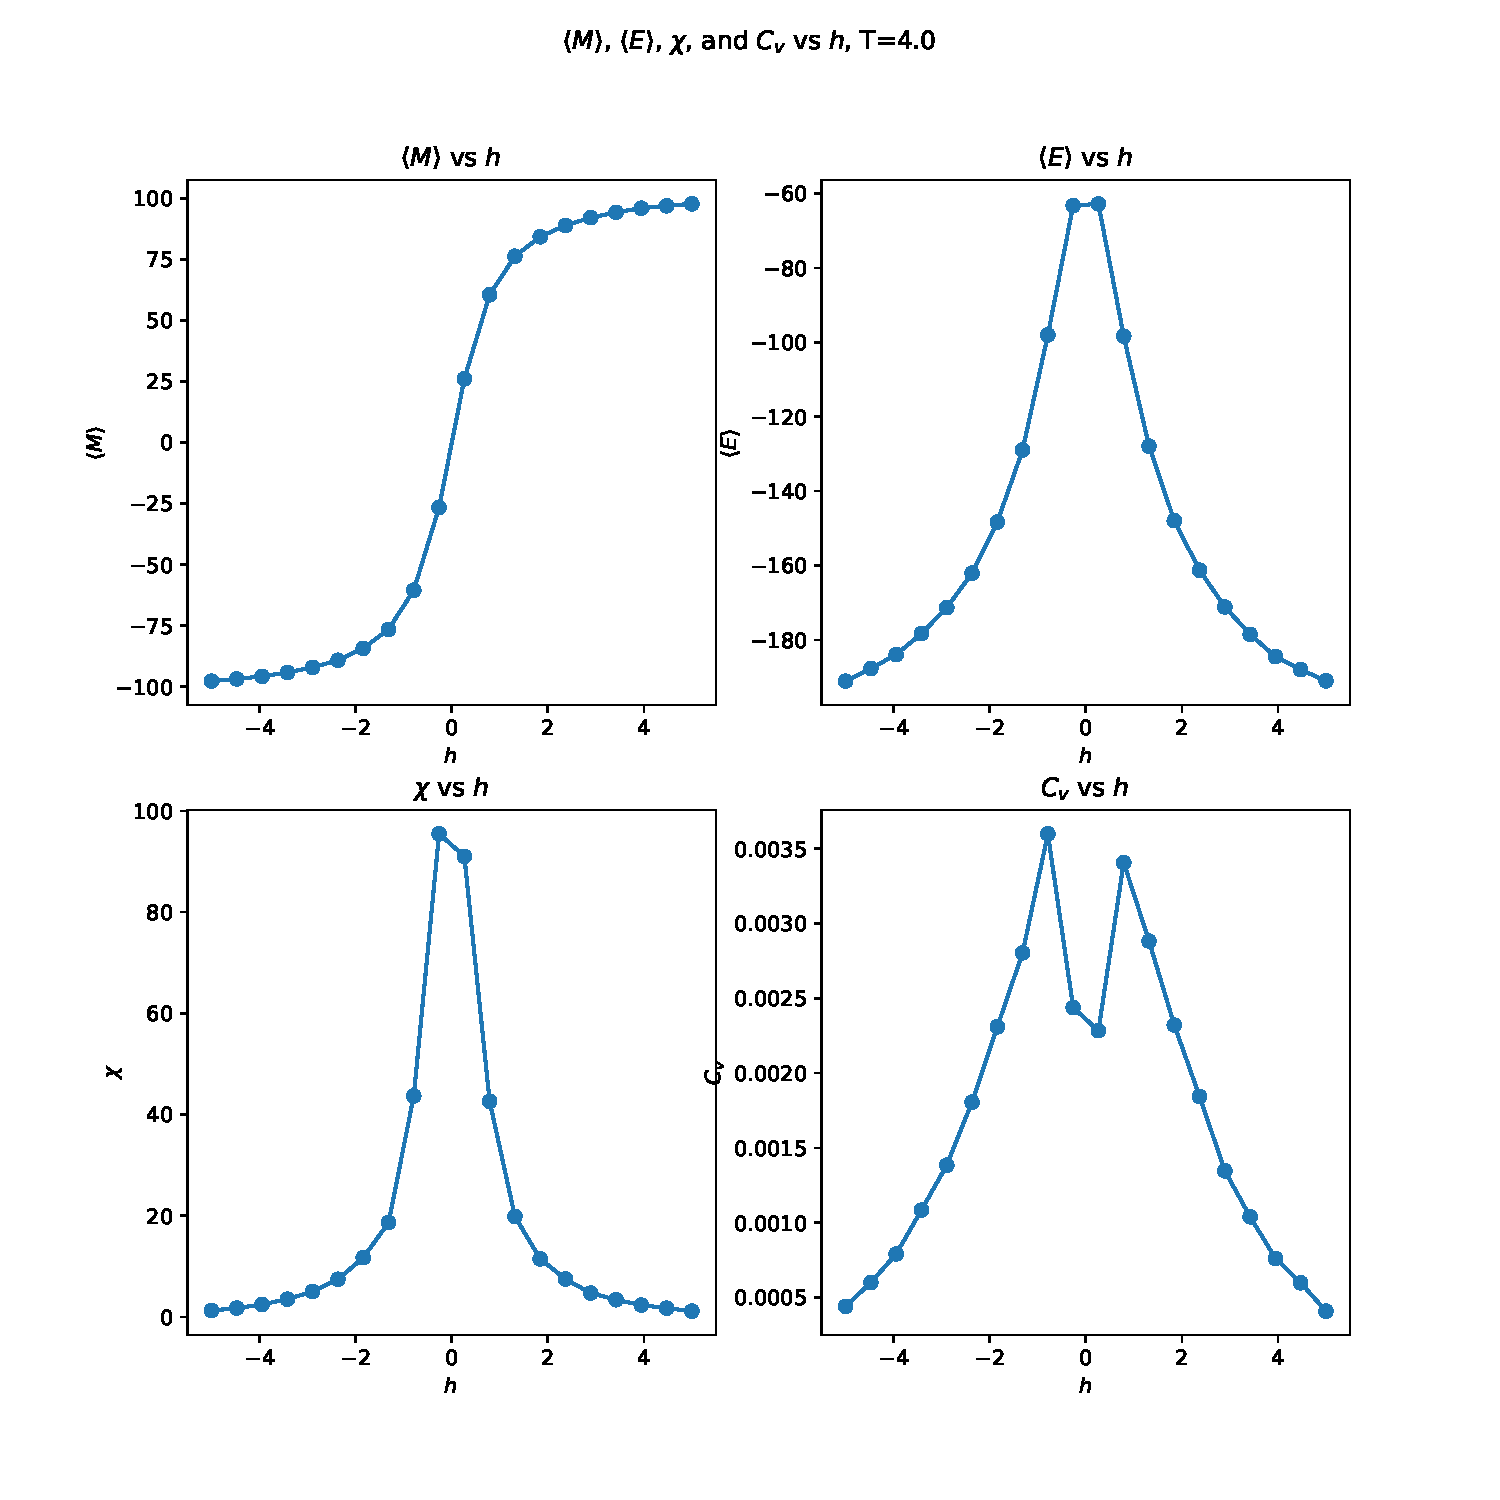
\includegraphics[width=0.5\textwidth]{h_graph_T=4.0.pdf} \\
    \end{tabular}
    \caption{\label{fig: h_graph_T=1.0,4.0}Magnetization, energy, heat capacity and magnetic susceptibility as a function of external field $h$ for $kT=1.0$, $L=10$}
    \end{flushleft}
\end{figure}
\indent The following result concerns the variables as functions of $kT$ for constant $h=0$, as in Fig.\ref{fig: T_graph_h=0}. $\braket{M}$ can take either a positive or negative value with equal likelihood, and so we can see the phase change from ferromagnetic to paramagnetic at the point where $\braket{M}$ drops toward zero ($\chi$ diverges). Since this phase change is continuous, we can also see it as the vanishing of the second derivative of the thermodynamic potential, $\braket{E}$, this point is the maximum of $C_v$, and the inflection of $\braket{E}$.
We estimate this point from the graph as being approximately $kT=2.3$.\\
\begin{figure}
    \centering
    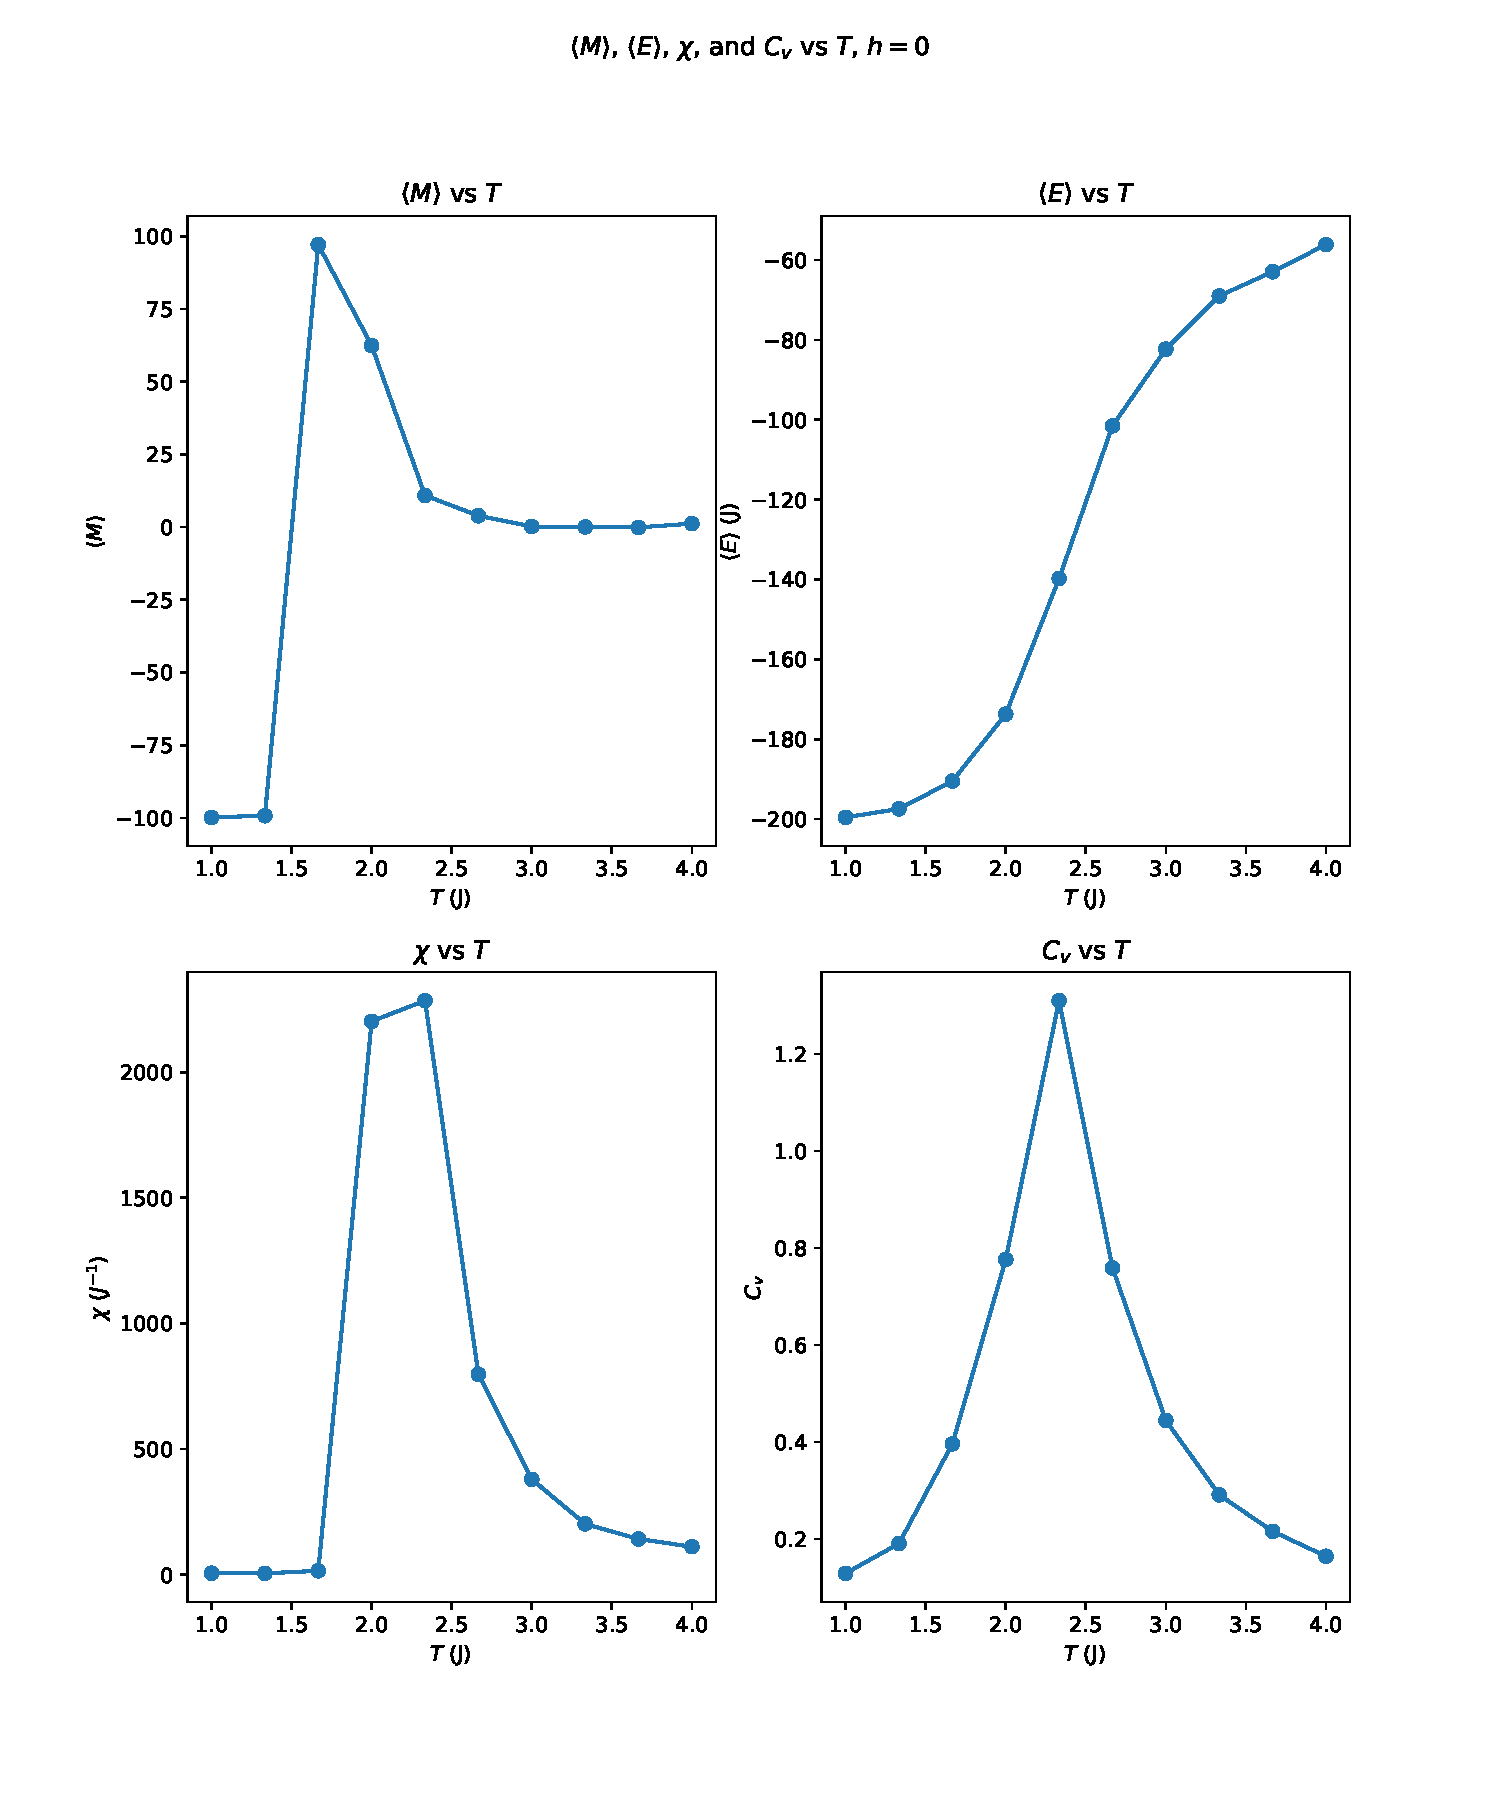
\includegraphics[width=0.6\textwidth]{T_graph_h=0.pdf}
    \caption{\label{fig: T_graph_h=0}Magnetization, energy, heat capacity and magnetic susceptibility as a function of temperature $kT$ for $h=0$, $L=10$}
\end{figure}
While an attempt was made to use plots of $\chi$ and $C_v$ as functions of system size, at the critical temperature, to estimate the critical exponents, the plots returned did not show the expected behaviour. This is likely caused by insufficient number of sweeps, or an error in the calculation of the variables.\\
\section{Conclusion}
In conclusion, the AI was able to generate a class for simulating the 2D Ising model, and the Metropolis algorithm. It did not however include methods for calculating more interesting variables, such as $C_v$ or $\chi$, nor any analysis of its method. I would conclude that the AI is capable of generating code for simple simulations, but is not capable of critiquing or analysing its own work to a sufficient level. In this fashion, I would say that the ability of the AI to generate code is limited significantly by both the standard of the code it is trained on, but also by the understanding of the one giving the prompt of both the physics concerned and the code itself.\\
In support of this, the AI is incapable of explaining the why the final plots did not show the expected behaviour, code which it itself generated.\\
\section{Prompts}
The prompts used for the AI were as follows:\\
\textit{`Generate a Python class to simulate the 2D Ising model on a square lattice using the Metropolis Monte Carlo algorithm'} Dec 14, 16:05, 2024\\
\textit{Now plot chi, $C_v$ as function of system size, for} $T=2.3, h=0$ Dec 16, 14:00, 2024 \\

\end{document}